\documentclass[aspectratio=169]{beamer}
\usetheme{Madrid}
\usecolortheme{default}

\usepackage{graphicx}
\usepackage{amsmath}
\usepackage{xcolor}
\usepackage{tikz}
\usepackage{pgfplots}

\definecolor{recon2color}{rgb}{0.8,0.2,0.1}
\definecolor{recon3color}{rgb}{0.1,0.5,0.2}

\pgfplotsset{compat=1.17}
\usetikzlibrary{patterns,arrows.meta}

\title{Functions as Vectors}
\subtitle{Discretization, inner product, orthonormal basis}
\author{CSE255 - Scalable Data Analysis}
\date{\today}

\begin{document}

\begin{frame}
  \titlepage
\end{frame}

% --- Intro ---
\begin{frame}{Functions as Vectors}
  \small
  Functions on an interval can be treated as \textbf{vectors}:
  \begin{itemize}
    \item Multiplying by a constant
    \item Adding two vectors
    \item Inner product, norm, orthogonality
    \item Representation in an orthonormal basis
  \end{itemize}
  \vspace{0.3cm}
  We use a \textbf{discrete grid} so we can compute and plot; in the continuous case sums become integrals.
\end{frame}

% --- Discretization ---
\begin{frame}{Functions as vectors (discretization)}
  \small
  A function $f$ is represented by its values $f(x)$ on the grid (a vector in $\mathbb{R}^d$).
  \vspace{0.15cm}
  \begin{columns}
    \column{0.62\textwidth}
  \begin{center}
    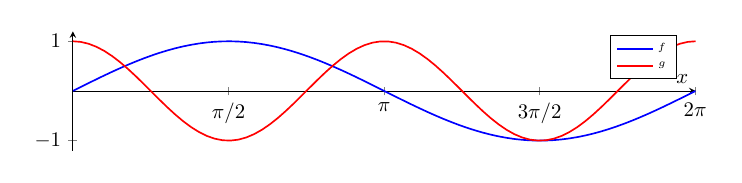
\begin{tikzpicture}[scale=0.75]
      \begin{axis}[
          width=\textwidth, height=3.6cm,
          xmin=0, xmax=2*pi, ymin=-1.2, ymax=1.2,
          axis lines=middle,
          xlabel={$x$}, ylabel={},
          xtick={0, 1.57, 3.14, 4.71, 6.28},
          xticklabels={0, $\pi/2$, $\pi$, $3\pi/2$, $2\pi$},
          legend pos=north east,
          legend style={font=\tiny}
        ]
        \addplot[blue, thick, domain=0:2*pi, samples=80] {sin(deg(x))};
        \addplot[red, thick, domain=0:2*pi, samples=80] {cos(deg(2*x))};
        \legend{$f$, $g$}
      \end{axis}
    \end{tikzpicture}
  \end{center}
  \textbf{Functions on the grid.}
    \column{0.35\textwidth}
  \textbf{2D analogue:}\\[0.2cm]
  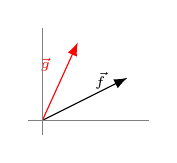
\begin{tikzpicture}[scale=0.9, every node/.style={font=\tiny}]
    \draw[-Latex] (0,0) -- (1.2,0.6) node[midway, above right] {$\vec{f}$};
    \draw[-Latex, red] (0,0) -- (0.5,1.1) node[midway, above left] {$\vec{g}$};
    \draw[gray, thin] (-0.2,0) -- (1.5,0) (0,-0.2) -- (0,1.3);
  \end{tikzpicture}
  Two vectors in $\mathbb{R}^2$.
  \end{columns}
\end{frame}

% --- Scalar multiplication ---
\begin{frame}{Scalar multiplication}
  \small
  $(c \cdot f)(x) = c \cdot f(x)$. Same as for vectors.
  \vspace{0.15cm}
  \begin{columns}
    \column{0.62\textwidth}
  \begin{center}
    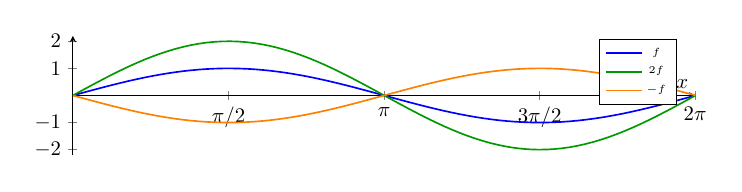
\begin{tikzpicture}[scale=0.75]
      \begin{axis}[
          width=\textwidth, height=3.6cm,
          xmin=0, xmax=2*pi, ymin=-2.2, ymax=2.2,
          axis lines=middle,
          xlabel={$x$}, ylabel={},
          xtick={0, 1.57, 3.14, 4.71, 6.28},
          xticklabels={0, $\pi/2$, $\pi$, $3\pi/2$, $2\pi$},
          legend pos=north east,
          legend style={font=\tiny}
        ]
        \addplot[blue, thick, domain=0:2*pi, samples=80] {sin(deg(x))};
        \addplot[green!60!black, thick, domain=0:2*pi, samples=80] {2*sin(deg(x))};
        \addplot[orange, thick, domain=0:2*pi, samples=80] {-sin(deg(x))};
        \legend{$f$, $2f$, $-f$}
      \end{axis}
    \end{tikzpicture}
  \end{center}
    \column{0.35\textwidth}
  \textbf{2D analogue:}\\[0.2cm]
  \begin{tikzpicture}[scale=0.9, every node/.style={font=\tiny}]
    \draw[-Latex, blue] (0,0) -- (1,0.5) node[right] {$\vec{f}$};
    \draw[-Latex, green!60!black] (0,0) -- (2,1) node[right] {$2\vec{f}$};
    \draw[-Latex, orange] (0,0) -- (-1,-0.5) node[left] {$-\vec{f}$};
    \draw[gray, thin] (-1.3,0) -- (2.2,0) (0,-0.7) -- (0,1.2);
  \end{tikzpicture}
  Scalar multiply: same direction, scaled length.
  \end{columns}
\end{frame}

% --- Addition ---
\begin{frame}{Addition}
  \small
  $(f + g)(x) = f(x) + g(x)$.
  \vspace{0.15cm}
  \begin{columns}
    \column{0.62\textwidth}
  \begin{center}
    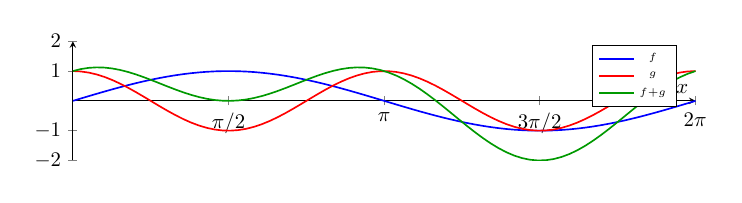
\begin{tikzpicture}[scale=0.75]
      \begin{axis}[
          width=\textwidth, height=3.6cm,
          xmin=0, xmax=2*pi, ymin=-2, ymax=2,
          axis lines=middle,
          xlabel={$x$}, ylabel={},
          xtick={0, 1.57, 3.14, 4.71, 6.28},
          xticklabels={0, $\pi/2$, $\pi$, $3\pi/2$, $2\pi$},
          legend pos=north east,
          legend style={font=\tiny}
        ]
        \addplot[blue, thick, domain=0:2*pi, samples=80] {sin(deg(x))};
        \addplot[red, thick, domain=0:2*pi, samples=80] {cos(deg(2*x))};
        \addplot[green!60!black, thick, domain=0:2*pi, samples=80] {sin(deg(x))+cos(deg(2*x))};
        \legend{$f$, $g$, $f{+}g$}
      \end{axis}
    \end{tikzpicture}
  \end{center}
    \column{0.35\textwidth}
  \textbf{2D analogue:}\\[0.2cm]
  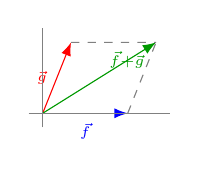
\begin{tikzpicture}[scale=0.9, every node/.style={font=\tiny}]
    \draw[-Latex, blue] (0,0) -- (1.2,0) node[midway, below] {$\vec{f}$};
    \draw[-Latex, red] (0,0) -- (0.4,1) node[midway, left] {$\vec{g}$};
    \draw[-Latex, green!60!black] (0,0) -- (1.6,1) node[midway, above right] {$\vec{f}{+}\vec{g}$};
    \draw[gray, dashed] (1.2,0) -- (1.6,1) (0.4,1) -- (1.6,1);
    \draw[gray, thin] (-0.2,0) -- (1.8,0) (0,-0.2) -- (0,1.2);
  \end{tikzpicture}
  Parallelogram rule: $\vec{f}+\vec{g}$.
  \end{columns}
\end{frame}

% --- Inner product ---
\begin{frame}{Inner product}
  \small
  \textbf{Discrete version} (approximates $\int f\,g$):
  \[
  \langle f, g \rangle = \sum_i f(x_i)\, g(x_i)\, \Delta x
  \]
  \textbf{Continuous case:} $\displaystyle \langle f, g \rangle = \int f(x)\, g(x)\, dx$.
  \vspace{0.3cm}
  Example: $\langle f,f \rangle$, $\langle g,g \rangle$, $\langle f,g \rangle$ are computed the same way as for vectors (with the weight $\Delta x$).
\end{frame}

% --- Norm ---
\begin{frame}{Norm}
  \small
  \[
  \|f\| = \sqrt{\langle f, f \rangle}
  \]
  Same as the length of the vector of samples, up to the factor $\sqrt{\Delta x}$.
\end{frame}

% --- Orthogonality ---
\begin{frame}{Orthogonality}
  \small
  Two functions are \textbf{orthogonal} if $\langle f, g \rangle = 0$.
  On $[0, 2\pi]$, $\sin(x)$ and $\cos(x)$ are orthogonal.
  \vspace{0.15cm}
  \begin{columns}
    \column{0.62\textwidth}
  \begin{center}
    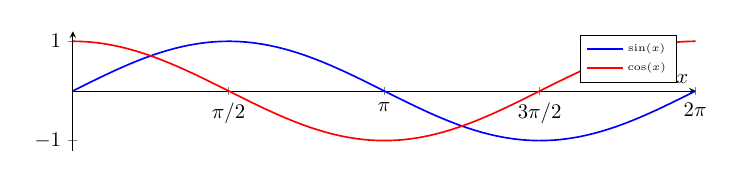
\begin{tikzpicture}[scale=0.75]
      \begin{axis}[
          width=\textwidth, height=3.6cm,
          xmin=0, xmax=2*pi, ymin=-1.2, ymax=1.2,
          axis lines=middle,
          xlabel={$x$}, ylabel={},
          xtick={0, 1.57, 3.14, 4.71, 6.28},
          xticklabels={0, $\pi/2$, $\pi$, $3\pi/2$, $2\pi$},
          legend pos=north east,
          legend style={font=\tiny}
        ]
        \addplot[blue, thick, domain=0:2*pi, samples=80] {sin(deg(x))};
        \addplot[red, thick, domain=0:2*pi, samples=80] {cos(deg(x))};
        \legend{$\sin(x)$, $\cos(x)$}
      \end{axis}
    \end{tikzpicture}
  \end{center}
  \textbf{Two orthogonal functions.}
    \column{0.35\textwidth}
  \textbf{2D analogue:}\\[0.2cm]
  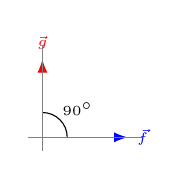
\begin{tikzpicture}[scale=0.9, every node/.style={font=\tiny}]
    \draw[-Latex, blue] (0,0) -- (1.2,0) node[right] {$\vec{f}$};
    \draw[-Latex, red] (0,0) -- (0,1.1) node[above] {$\vec{g}$};
    \draw (0.35,0) arc (0:90:0.35);
    \node at (0.5,0.4) {$90^\circ$};
    \draw[gray, thin] (-0.2,0) -- (1.4,0) (0,-0.2) -- (0,1.3);
  \end{tikzpicture}
  $\vec{f}\cdot\vec{g}=0$: perpendicular.
  \end{columns}
\end{frame}

% --- Orthonormal basis ---
\begin{frame}{Orthonormal basis}
  \small
  A set $\{u_1, \ldots, u_k\}$ is \textbf{orthonormal} if $\|u_i\| = 1$ and $\langle u_i, u_j \rangle = 0$ for $i \neq j$.
  \vspace{0.2cm}
  Then any $f$ in their span can be written
  \[
  f = \sum_i c_i u_i \quad \text{with} \quad c_i = \langle f, u_i \rangle.
  \]
  \vspace{0.2cm}
  Example on $[0, 2\pi]$: $u_0 = \frac{1}{\sqrt{2\pi}}$, $u_1 = \frac{\cos(x)}{\sqrt{\pi}}$, $u_2 = \frac{\sin(x)}{\sqrt{\pi}}$ (normalized so discrete norms are 1). Then $\langle u_i, u_j \rangle = \delta_{ij}$.
\end{frame}

% --- Representation ---
\begin{frame}{Representation using the orthonormal basis}
  \small
  Coefficients: $c_i = \langle f, u_i \rangle$. Reconstruction: $f_{\text{recon}} = \sum_i c_i u_i$ (1, 2, or 3 terms).
  If $f$ lies in the span of $\{u_i\}$, reconstruction is exact; otherwise best approximation.
  \vspace{0.15cm}
  \begin{columns}
    \column{0.62\textwidth}
  \begin{center}
    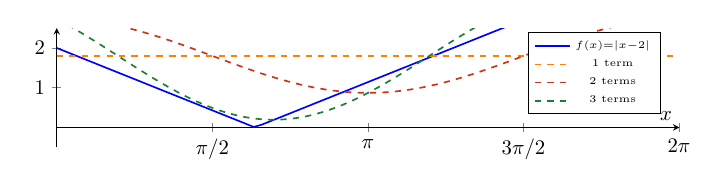
\begin{tikzpicture}[scale=0.75]
      \begin{axis}[
          width=\textwidth, height=3.6cm,
          xmin=0, xmax=2*pi, ymin=-0.5, ymax=2.5,
          axis lines=middle,
          xlabel={$x$}, ylabel={},
          xtick={0, 1.57, 3.14, 4.71, 6.28},
          xticklabels={0, $\pi/2$, $\pi$, $3\pi/2$, $2\pi$},
          legend pos=north east,
          legend style={font=\tiny}
        ]
        \addplot[blue, thick, domain=0:2*pi, samples=80] {abs(x-2)};
        \addplot[orange, thick, dashed, domain=0:2*pi, samples=80] {1.8};
        \addplot[recon2color, thick, dashed, domain=0:2*pi, samples=80] {1.8 + 0.93*cos(deg(x))};
        \addplot[recon3color, thick, dashed, domain=0:2*pi, samples=80] {1.8 + 0.93*cos(deg(x)) - 1.31*sin(deg(x))};
        \legend{$f(x){=}|x{-}2|$, 1 term, 2 terms, 3 terms}
      \end{axis}
    \end{tikzpicture}
  \end{center}
  $f(x)=|x-2|$: best approximation with 1, 2, or 3 basis functions $\{1,\cos,\sin\}$.
    \column{0.35\textwidth}
  \textbf{2D analogue:}\\[0.2cm]
  Rotated orthonormal basis $\vec{u}_1$, $\vec{u}_2$.\\
  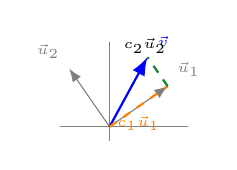
\begin{tikzpicture}[scale=0.9, every node/.style={font=\tiny}]
    \draw[gray, thin] (-0.7,0) -- (1.1,0) (0,-0.2) -- (0,1.2);
    % Orthonormal: u1 = (0.82, 0.57), u2 = (-0.57, 0.82), u1·u2 = 0
    \draw[-Latex, gray] (0,0) -- (0.82,0.57) node[above right] {$\vec{u}_1$};
    \draw[-Latex, gray] (0,0) -- (-0.57,0.82) node[above left] {$\vec{u}_2$};
    % v = c1*u1 + c2*u2 with c1=1, c2=0.5 => v = (0.535, 0.98); c1*u1 ⊥ c2*u2
    \draw[-Latex, blue, thick] (0,0) -- (0.535,0.98) node[above right] {$\vec{v}$};
    % 1 term: c1*u1 (projection onto u1), parallel to u1
    \draw[orange, dashed, thick] (0,0) -- (0.82,0.57) node[midway, below] {$c_1\vec{u}_1$};
    % 2 terms: add c2*u2 (parallel to u2, hence ⊥ to c1*u1)
    \draw[recon3color, dashed, thick] (0.82,0.57) -- (0.535,0.98);
    \node at (0.5,0.9) [above] {\tiny $c_2\vec{u}_2$};
  \end{tikzpicture}
  1 term: $c_1\vec{u}_1$. 2 terms: $c_1\vec{u}_1+c_2\vec{u}_2$; $c_1\vec{u}_1\perp c_2\vec{u}_2$.
  \end{columns}
\end{frame}

% --- Recap ---
\begin{frame}{Recap}
  \small
  Functions on an interval can be seen as vectors. We demonstrated:
  \begin{itemize}
    \item \textbf{Scalar multiplication} and \textbf{addition}
    \item \textbf{Inner product} (discrete sum approximating an integral)
    \item \textbf{Norm} $\|f\| = \sqrt{\langle f,f \rangle}$
    \item \textbf{Orthogonality} $\langle f,g \rangle = 0$
    \item \textbf{Orthonormal basis} and \textbf{representation} $f = \sum_i c_i u_i$ with $c_i = \langle f, u_i \rangle$
  \end{itemize}
  \vspace{0.2cm}
  In the continuous case, sums are replaced by integrals.
\end{frame}

\end{document}
